%%%%%%%%%%%%%%%%%%%%%%%%%%%%%%%%%%%%%%%%%%%%%%%%%%%%%%%%%%%%%%%%%%%%%%
%%
%% This LaTeX file typesets the User's Guide for fbe_tez.sty.
%%
%%%%%%%%%%%%%%%%%%%%%%%%%%%%%%%%%%%%%%%%%%%%%%%%%%%%%%%%%%%%%%%%%%%%%%
%%
%% COPYRIGHT 1999, 2001, 2003 by
%% Feza Kerestecioglu <kerestec@boun.edu.tr>
%%
%% Copying of part or all of any file in the fbe_tez package is
%% allowed under the following conditions only:
%% (1) You may freely distribute unchanged copies of the files. Please
%%     include the documentation when you do so.
%% (2) You may modify a renamed copy of any file, but only for your
%%     personal use.
%% (3) You may copy fragments from the files, for personal use only
%%     and as long as credit is given where credit is due.
%%
%% You are NOT ALLOWED to take money for the distribution or use of
%% these files or modified versions or fragments thereof.
%%
%%%%%%%%%%%%%%%%%%%%%%%%%%%%%%%%%%%%%%%%%%%%%%%%%%%%%%%%%%%%%%%%%%%%%%
%

\documentclass[12pt]{article}
\usepackage{float}
%\usepackage[bottom]{footmisc}
\usepackage{cite}
\usepackage{graphicx}
\usepackage{longtable}
\graphicspath{{figures/}} % Graphics will be here

%
% Pagestyle
%
\oddsidemargin9.6mm
\evensidemargin9.6mm
\topmargin-1cm
\headheight20pt
\textwidth155mm
\textheight232mm
\pagestyle{myheadings}
%
% Macros
%
\newcommand\fbe{{\tt fbe\_tez}}
\newcommand\report{{\tt report}}
\newcommand{\bq}{\begin{quotation}\noindent}
\newcommand{\eq}{\end{quotation}}
\renewcommand{\arg}[1]{$\langle\mbox{\it #1}\rangle$}
%
% Title declarations
%

\title{{\Huge CmpE 443 Final Project Design Document} \\ Group Name: Tezla  }
\author{Members \\ Abdurrahman DILMAC (Team Leader) \\ Ahmet Semih ARI\\ Ramazan ARSLAN\\ Yunus Emre DEMIRCI}
\date{November 21, 2018 \\ Version 1.00}
%
\begin{document}
\maketitle
\tableofcontents
\newpage
\section{System Level Structural Diagram (Block Diagram)}

\begin{figure}[htbp]
\begin{center}
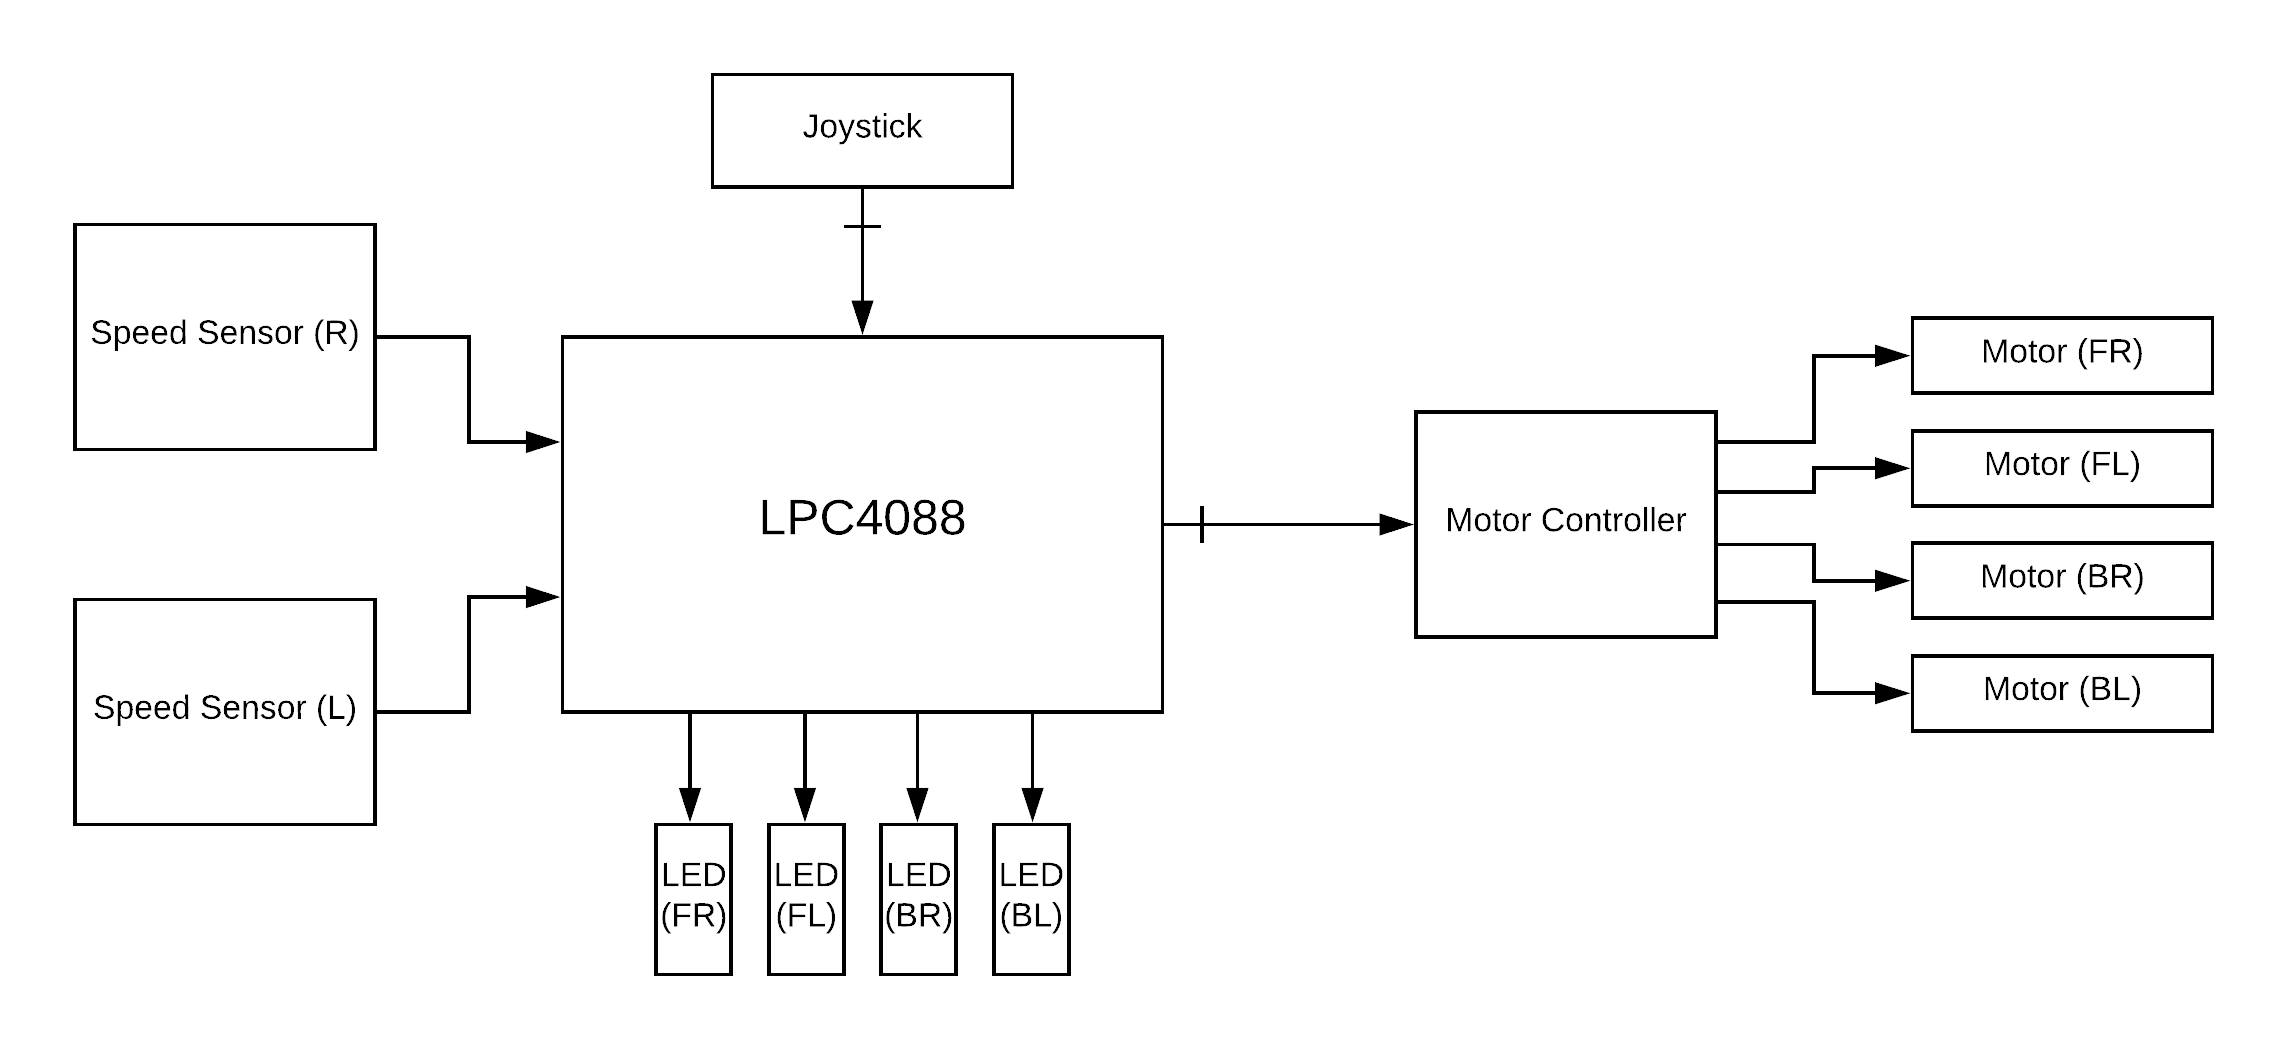
\includegraphics[width=1\columnwidth]{structure-diagram.png}
\end{center}
\caption{Block Diagram of car.}
\vskip\baselineskip % Leave a vertical skip below the figure
\label{fig:sample}
\end{figure}

\textbf{LPC4088 Microcontroller:} Main part of the car. Runs software and controls peripherals.

\textbf{Motor Speed Sensor:} Used to measure motor speed by counting holes. It's used to first, to detect speed and the second, getting feedback on turn angle of the car.

\textbf{Motor controller:} By getting inputs from the main board, controls motors by means of controlling speed, directions, soft and hard brakes.

\textbf{Motor:} Gives tork to the car, and thus moves.

\textbf{LEDs:} Emits light, controlled by the main board. Used for car signals.

\textbf{Joystick:} Takes input from the player/user and informs the main board, so it can take appropriate action.


\newpage
\section{Sequence Diagram}

\begin{figure}[htbp]
\begin{center}
\hspace*{-1.1in}
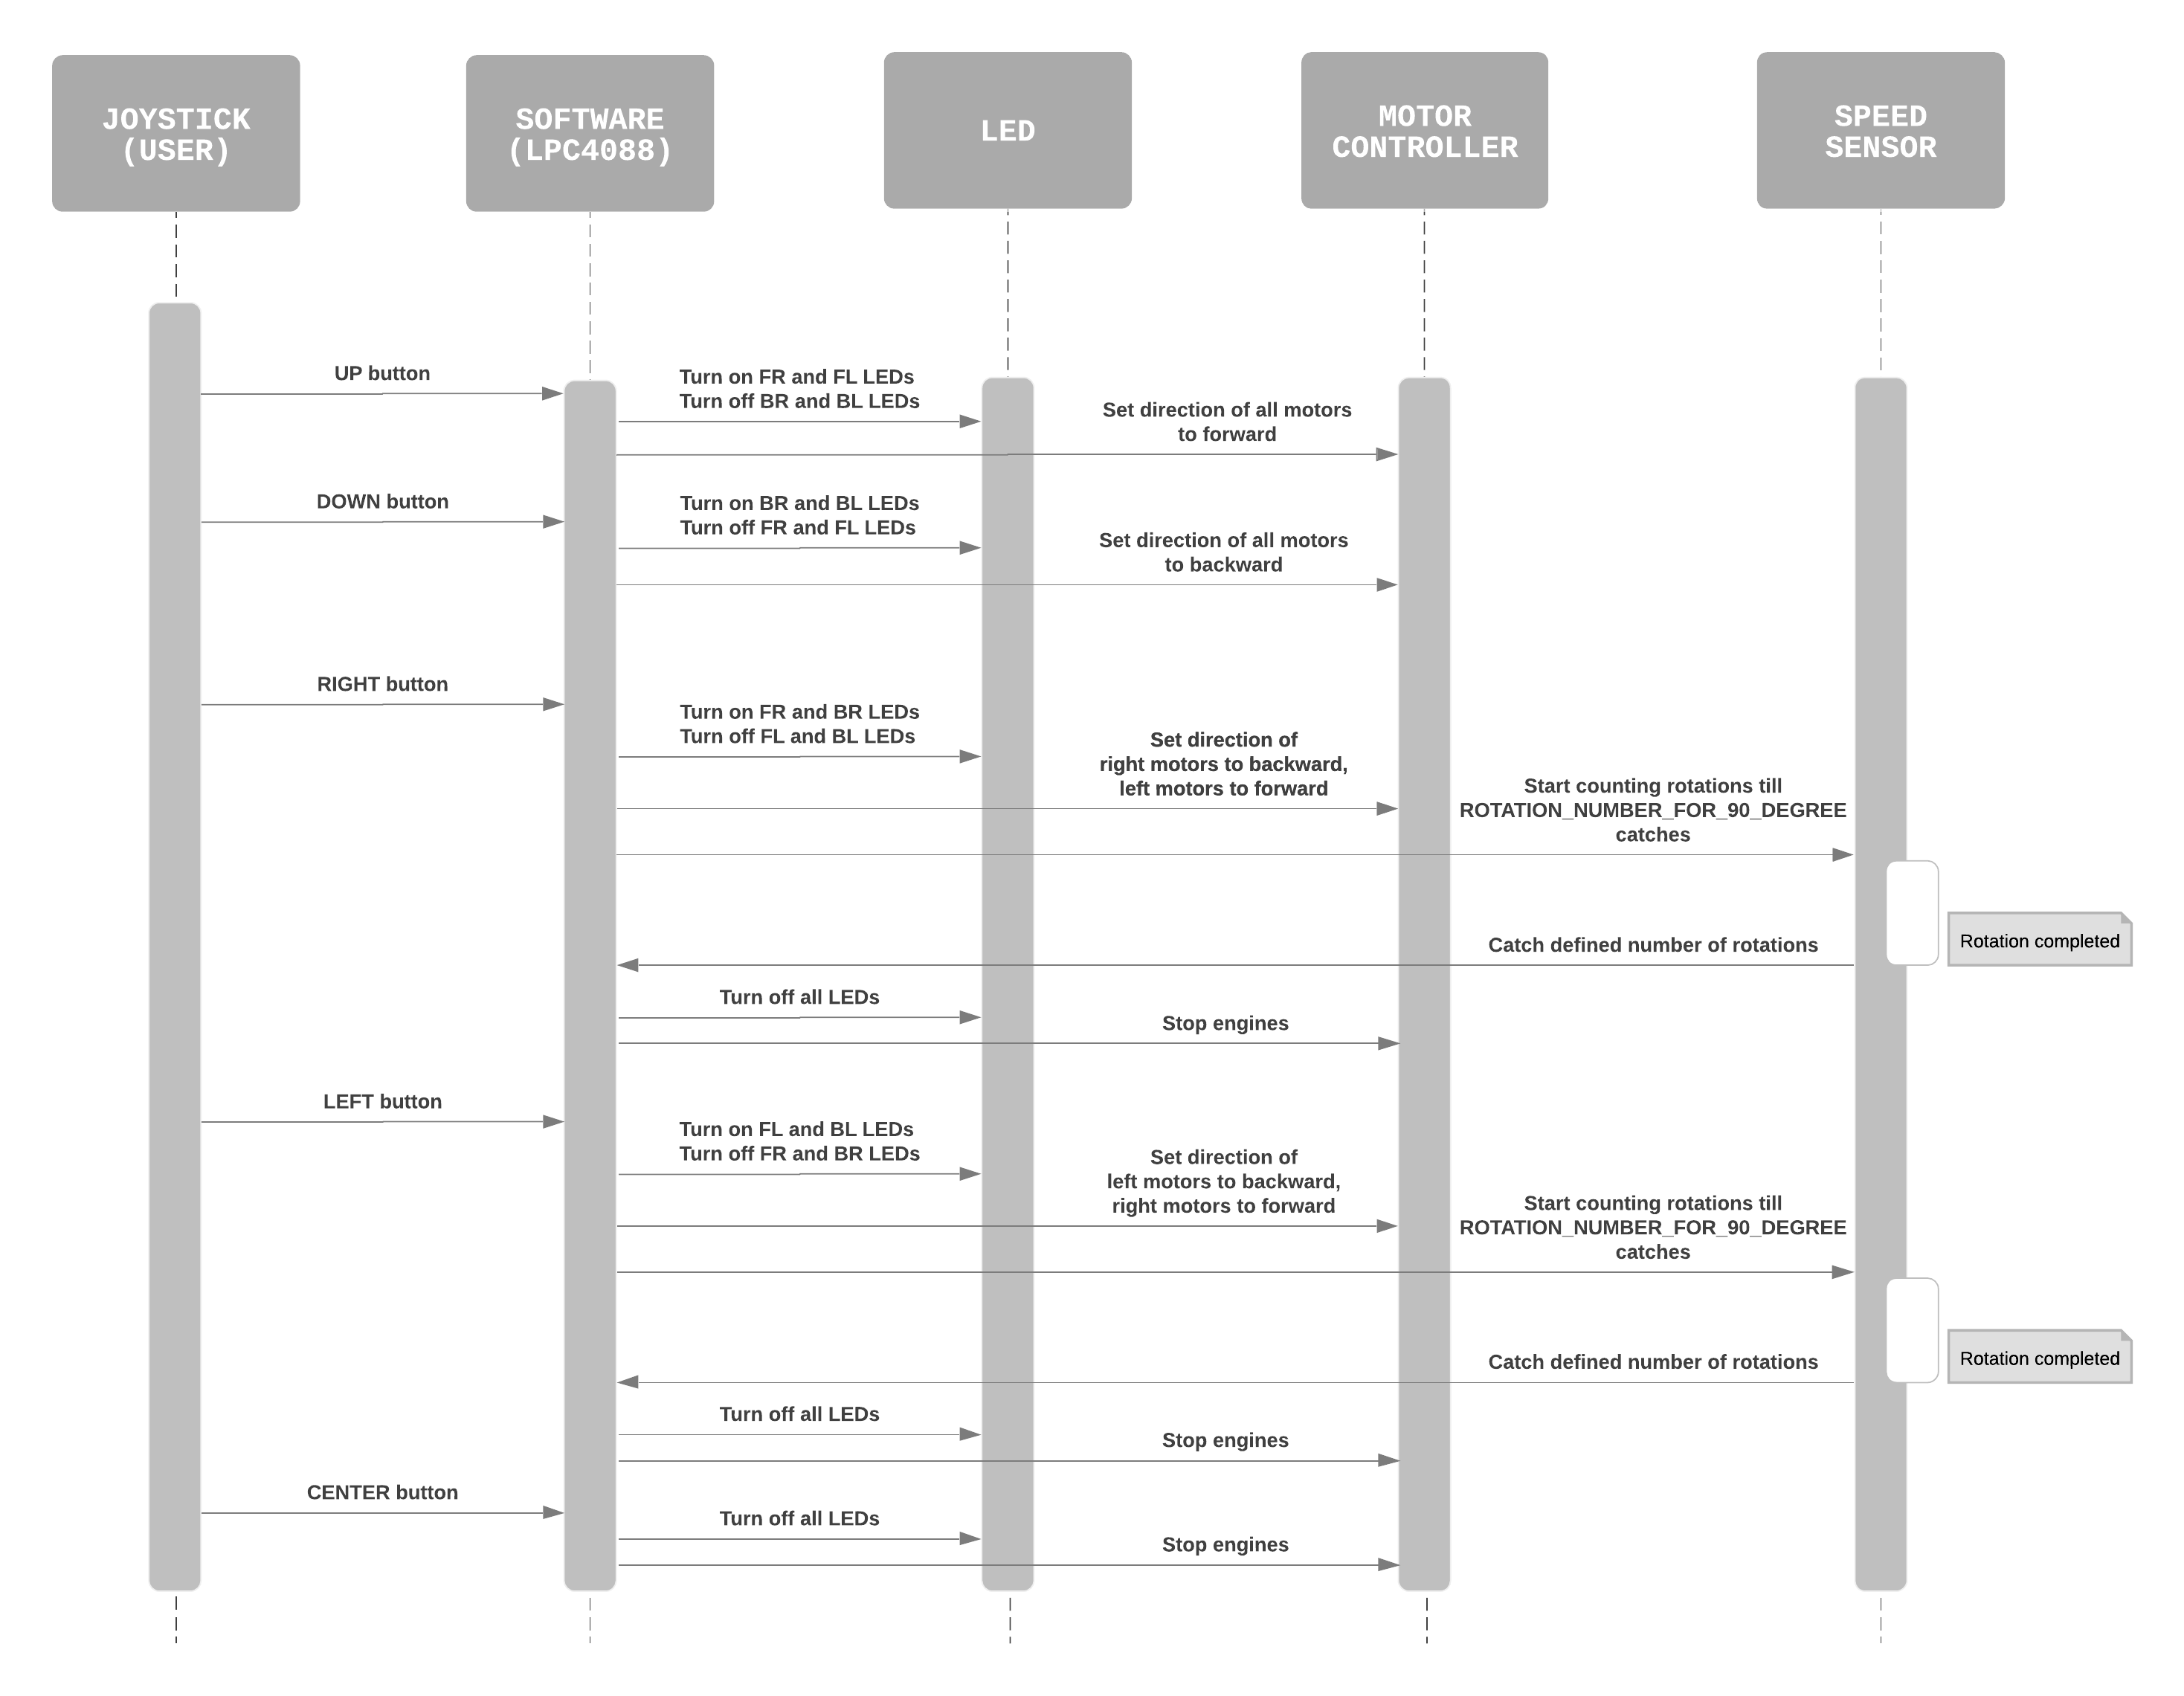
\includegraphics[width=1.30\columnwidth]{sequence-diagram-dark.png}
\end{center}
\caption{Sequence Diagram.}
\vskip\baselineskip % Leave a vertical skip below the figure
\label{fig:sample}
\end{figure}


\newpage
\section{LED Connections}

All the components which are controlled via LPC4088 should be connected to the board. Therefore, you should determine the pins and their functionalities. Draw the described table in the term project interim report description document. After you determine the all the pins, draw the circuit schematic for the LED circuits. \\

\begin{center}
\begin {table}[H]
\begin{tabular}{|c|c|c|c|c|}
\hline
The LED name & LPC4088 PIN & Port & Pin Functionality & Reason \\\hline
Front Right LED & PIN5 & P1.24 & GPIO & Supports digital I/O \\\hline
Front Left LED & PIN6 & P1.23 & GPIO & Supports digital I/O \\\hline
Back Right LED & PIN7 & P1.20 & GPIO & Supports digital I/O \\\hline
Back Left LED & PIN8 & P0.21 & GPIO & Supports digital I/O \\\hline
\end{tabular}
\caption{LED Pins and their functionalities}
\end{table}
\end{center}


\begin{figure}[htbp]
\begin{center}
%\hspace*{-1in}
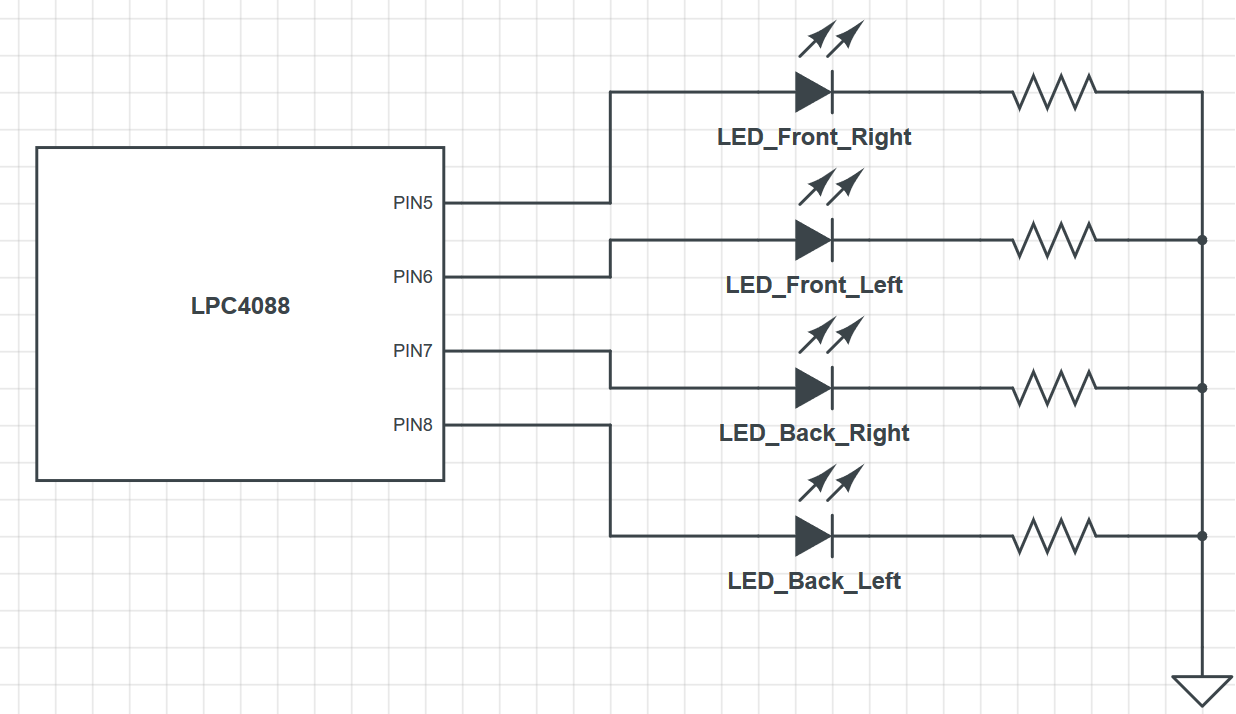
\includegraphics[width=1\columnwidth]{led-circuit-diagram.png}
\end{center}
\caption{LED Circuit Diagram.}
\vskip\baselineskip % Leave a vertical skip below the figure
\label{fig:sample}
\end{figure}

\newpage
\section{Motor - Speed Sensor Connection}

\begin {table}[H]
\begin{center}
\begin{tabular}{|c|c|c|c|c|}
\hline
Speed sensor PIN & LPC4088 PIN & Port & Pin Functionality & Reason \\\hline
Power GND & PIN1 & GND & Ground & Ground is needed \\\hline
VCC & PIN44 & VU & Power input & For transferring voltage \\\hline
\shortstack{Right\\ Speed Sensor \\OUT} & PIN15 & P0.23 & T3\_CAP\_0 & \shortstack{Supports\\ Timer functionality} \\\hline
\shortstack{Left\\ Speed Sensor \\OUT} & PIN34 & P1.4 & T2\_CAP\_0 & \shortstack{Supports\\ Timer functionality} \\\hline
\end{tabular}
\caption{Motor Driver and board PIN connections with their functionalities.}
\end{center}
\end{table}

Even though two different speed sensors said to be used in the project description, our implementation can work with only one speed sensor for this part of the project. So, Left is connected to the board by design, but not needed and thus not used.


\newpage
\section{Motor - Driver Connection}

There is only one motor controller to control 4 motors. Output A is used for right motors and Output B is for left motors.

\begin {table}[H]
\begin{center}
\begin{tabular}{|c|c|}
\hline
Motor Terminal & Motor Driver Terminal \\\hline
Motor 1 + & Output A + \\\hline
Motor 1 - & Output A - \\\hline
Motor 2 + & Output A + \\\hline
Motor 2 - & Output A - \\\hline
Motor 3 + & Output B + \\\hline
Motor 3 - & Output B - \\\hline
Motor 4 + & Output B + \\\hline
Motor 4 - & Output B - \\\hline
\end{tabular}
\caption{Motor Driver and motor connections.}
\end{center}
\end{table}


\newpage
\section{Driver - Board Connection}

Here is the table depicting relations between the board and motor controller:

\begin {table}[H]
\begin{center}
\begin{tabular}{|c|c|c|c|c|}
\hline
Motor driver PIN & LPC4088 PIN & Port & Pin Functionality & Reason \\\hline
Power GND & PIN1 & GND & Ground & Ground is needed \\\hline
+5V Power & PIN44 & Vout & Power input & For transferring voltage \\\hline
A Enable & PIN29 & P1.3 & PWM0\_1 (ENA) & Supports PWM Output \\\hline
B Enable & PIN30 & P1.2 & PWM0\_2 (ENB) & Supports PWM Output \\\hline
Logic Input 1 & PIN12 & P0.8 & GPIO & Supports digital I/O \\\hline
Logic Input 2 & PIN11 & P0.9 & GPIO & Supports digital I/O \\\hline
Logic Input 3 & PIN16 & P0.24 & GPIO & Supports digital I/O \\\hline
Logic Input 4 & PIN13 & P0.7 & GPIO & Supports digital I/O \\\hline
\end{tabular}
\caption{Motor Driver and board PIN connections with their functionalities.}
\end{center}
\end{table}


\end{document}
%
% End of fbeman.tex
